% Join of fixed points p and q is j in the lattice, and t among fixed points.
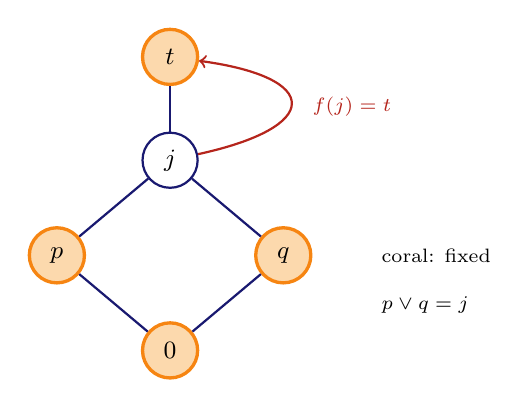
\begin{tikzpicture}[x=1.25cm,y=1.05cm,
  fix/.style={circle,draw=BurntOrange,line width=1.2pt,fill=BurntOrange!28,inner sep=1.5pt,minimum size=7mm,font=\small},
  mov/.style={circle,draw=MidnightBlue,thick,fill=white,inner sep=1.5pt,minimum size=7mm,font=\small}]
  \node[fix] (z) at (0,0) {$0$};
  \node[fix] (p) at (-1.15,1.15) {$p$};
  \node[fix] (q) at (1.15,1.15) {$q$};
  \node[mov] (j) at (0,2.3) {$j$};
  \node[fix] (t) at (0,3.55) {$t$};
  \draw[MidnightBlue,thick] (z) -- (p);
  \draw[MidnightBlue,thick] (z) -- (q);
  \draw[MidnightBlue,thick] (p) -- (j);
  \draw[MidnightBlue,thick] (q) -- (j);
  \draw[MidnightBlue,thick] (j) -- (t);
  \draw[BrickRed,thick,->] (j) .. controls (1.55,2.7) and (1.55,3.3) .. (t);
  \node[font=\scriptsize,BrickRed,anchor=west] at (1.35,2.95) {$f(j)=t$};
  \node[font=\scriptsize,anchor=west,align=left] at (2.05,1.15) {coral: fixed};
  \node[font=\scriptsize,anchor=west,align=left] at (2.05,0.55) {$p\lor q=j$};
\end{tikzpicture}
